% =============================================================================
% main.tex — Sparsity-TravelWise, condensed 10-page manual.
% Compile: pdflatex main && bibtex main && pdflatex main && pdflatex main
% =============================================================================
\documentclass[11pt,a4paper]{article}
% latex-shortened/preamble.tex
% Lean preamble for the 10-page condensed manual.
% Target: pdflatex on Overleaf free tier or local TeX Live, single pass < 10 s.

\usepackage[utf8]{inputenc}
\usepackage[T1]{fontenc}
\usepackage[margin=1in]{geometry}

% Allow long teletype identifiers (e.g. \texttt{prev\_stop\_actual\_delay})
% to break across lines without overfull boxes.
\setlength{\emergencystretch}{2em}
\hyphenpenalty=1000
\tolerance=2000

% Maths
\usepackage{amsmath, amssymb}

% Figures + sub-figures + [H] floats
\usepackage{graphicx}
\usepackage{subcaption}
\usepackage{float}
% Break long monospace identifiers (Maven coords, snake_case column lists)
% inside \texttt{} via \seqsplit{...}.
\usepackage{seqsplit}
\usepackage{caption}
\captionsetup[figure]{font=small, labelfont=bf, justification=raggedright,
                       singlelinecheck=false}
\captionsetup[table]{font=small, labelfont=bf, justification=raggedright,
                      singlelinecheck=false}

% Tables
\usepackage{booktabs}
\usepackage{array, tabularx}
\usepackage{siunitx}
% round-mode=none: \num{x} renders x verbatim with thousand-separator grouping
% only — no ".000" padding on plain integers in prose. Per-cell rounding can
% still be turned on inside individual S columns when needed.
\sisetup{detect-weight=true, detect-family=true,
          group-separator={,}, group-minimum-digits=4,
          round-mode=none}

% Bibliography
\usepackage[numbers, sort&compress, square]{natbib}
\bibliographystyle{plainnat}

% Hyperlinks (xcolor must precede so `blue!60!black` mixing works;
% cleveref must come AFTER hyperref).
\usepackage{xcolor}
\usepackage[colorlinks=true,
            linkcolor=blue!60!black,
            citecolor=blue!60!black,
            urlcolor=blue!60!black]{hyperref}
\usepackage[capitalise, noabbrev]{cleveref}

% Lists, paragraph spacing
\usepackage{enumitem}
\setlist{nosep, leftmargin=*}
\usepackage{parskip}

% Compact section headings to save vertical space.
\usepackage{titlesec}
\titlespacing*{\section}{0pt}{0.8\baselineskip}{0.3\baselineskip}
\titlespacing*{\subsection}{0pt}{0.5\baselineskip}{0.2\baselineskip}

% Graphics path: pull figures from the parent project rather than copy.
% Paths are RELATIVE to latex-shortened/.
\graphicspath{{../latex/figures/}{../stop_level/figures/}}


\title{\bfseries Stop-Level Disruption Prediction for IT/FI/NL Railways:\\
        \large A Ten-Page Manual to the Pipeline, Models, XAI and Knowledge Graph}
\author{Anonymous Authors\\\small\href{https://github.com/Zhiqian-Zhou/Sparsity-TravelWise}{\texttt{github.com/Zhiqian-Zhou/Sparsity-TravelWise}}}
\date{May 2026}

\begin{document}
\maketitle

\begin{abstract}
\small
We harmonise \num{16600169} stop rows from three open European railway feeds (Italy, Finland, Netherlands; Jan--Jun 2024) into a single anti-leakage Common Data Model with 37 (pre-departure) or 40 (inflight) features, and benchmark four model families twice on identical splits. The strongest pre-departure model (XGBoost) reaches test PR-AUC \num{0.527}; the inflight variant reaches \num{0.939}, with a lag-feature ablation showing the entire uplift is carried by lag and inflight features (collapse to PR-AUC \num{0.350} without them). On the Dutch labelled cause-of-disruption set the multi-class classifier reaches macro-F1 \num{0.213}, with the rare \emph{weather} class at F1$=$\num{0.509} thanks to a \texttt{winter\_x\_severe\_weather} interaction. A Sparksee 5.2.3 knowledge graph closes the loop from SHAP attribution to spatial-temporal context in \SI{7.7}{ms}. The full pipeline is reproducible from raw data with four shell commands and runs end-to-end in $\sim$1.5\,h on a multi-core host. This document is a manual: every load-bearing number, every model, every figure path is here.
\end{abstract}

\section{Overview}
\label{sec:overview}

\paragraph{Problem.} For every scheduled stop of every passenger train in Italy, Finland and the Netherlands (Jan--Jun 2024; \num{16600169} stops, \num{1559006} services, \num{2398} stations) predict $P(\text{disrupted})$, where a stop is \emph{disrupted} if its arrival is more than five minutes late or it is cancelled. About \SI{8.66}{\percent} of test-month stops meet that criterion, so the operationally relevant baseline is the per-class precision-recall trade-off, not accuracy.

\paragraph{Two operational scenarios.} Each model is trained twice on identical splits.
\begin{itemize}
    \item \textbf{Scenario A -- pre-departure.} 37 features. Available before the train leaves the platform: timetable, station-static, weather, lagged history. Use case: day-ahead planning and passenger alerts.
    \item \textbf{Scenario B -- inflight.} 40 features. Adds three columns describing actual delays at \emph{prior} stops on the same run: \texttt{prev\_stop\_actual\_delay}, \texttt{cum\_actual\_delay\_so\_far}, \texttt{max\_actual\_delay\_so\_far}. Use case: live retiming and propagation forecast.
\end{itemize}

\paragraph{Pipeline phases.} Each phase owns its own artefacts; downstream phases need only the previous phase's outputs.

\begin{enumerate}
    \item Raw download (\texttt{scripts/download\_data.sh}) $\to$ \SI{5.7}{GB} on disk.
    \item Per-country preprocessing (\texttt{preprocess/run\_all\_notebooks.sh}) $\to$ five standardised CSVs per country (\texttt{nodes\_station, nodes\_service, edges\_stops\_at, edges\_adjacent, nodes\_fault}).
    \item Unified stop store (\texttt{stop\_level/preprocess\_stops.py}) $\to$ \texttt{Data/stops/*.parquet} + scaler + graph tensors + \texttt{feature\_names\_\{A,B\}.json} + \texttt{manifest\_stops.json}.
    \item Model zoo (\texttt{stop\_level/train\_all.py --model logreg lgbm xgb graphsage --scenario both}) $\to$ per-(model, scenario) pickles + prediction parquets.
    \item Evaluation (\texttt{stop\_level/evaluate.py}) $\to$ 8 figures + \texttt{benchmark\_stops.json}.
    \item Explainability (\texttt{stop\_level/xai\_stops.py}) $\to$ 14 SHAP figures + \texttt{xai\_report\_stops.json} + lag-ablation refit.
    \item Knowledge graph (\texttt{stop\_level/build\_kg.py}) $\to$ Sparksee~5.2.3 graph + bridge-query demo.
    \item Cause classifier (\texttt{stop\_level/cause\_pred/run\_all.py}) $\to$ Dutch macro-F1 + cross-country transfer audit.
\end{enumerate}

\paragraph{Five contributions.} (i)~A unified anti-leakage feature store covering three operators (\cref{sec:data}). (ii)~A four-model benchmark trained twice (logreg, LightGBM~\cite{ke2017lightgbm}, XGBoost~\cite{chen2016xgboost}, GraphSAGE~\cite{hamilton2017inductive}) with the inflight uplift dominated by one feature (\cref{sec:models}). (iii)~TreeSHAP~\cite{lundberg2017unified,lundberg2020local} attributions plus a lag-feature ablation that decomposes the uplift cleanly (\cref{sec:xai}). (iv)~A Sparksee~\cite{sparksee2024} knowledge graph that takes a SHAP-flagged $(\texttt{service}, \texttt{station}, \texttt{date})$ triple and returns surrounding context in \SI{7.7}{ms} (\cref{sec:kgcause}). (v)~A multi-class cause-of-disruption classifier on Dutch labels reaching macro-F1 \num{0.213}, with documented cross-country transfer failure modes and recommended fixes (\cref{sec:kgcause}).

\section{Data, features, anti-leakage}
\label{sec:data}

\subsection{Three feeds, one Common Data Model}

The three operators share almost no schema. Italy publishes a flat per-stop CSV that encodes ``no upstream delay'' as the literal string \texttt{N} and ``cancelled'' as \texttt{S}. Finland publishes one row per train with every stop nested in a serialised Python literal carrying embedded FMI weather observations. The Netherlands publishes wide-tariff RDT exports with three separate cancellation flags and no built-in weather (we enrich it with Open-Meteo daily aggregates). After per-country preprocessing every country's \texttt{processed/} folder contains the same five tables (\texttt{nodes\_station, nodes\_service, edges\_stops\_at, edges\_adjacent, nodes\_fault}), which Phase~2 joins at the stop level.

\begin{table}[H]
    \centering
    \caption{Per-country scale after Phase~1, Jan--Jun~2024. Stops in millions, services in thousands; exact counts: 16{,}600{,}169 stops, 1{,}559{,}006 services, 2{,}398 stations.}
    \label{tab:data-sources}
    \footnotesize
    \setlength{\tabcolsep}{8pt}
    \begin{tabularx}{\textwidth}{l X
        S[table-format=2.2, round-mode=places, round-precision=2]
        S[table-format=4.1, round-mode=places, round-precision=1]
        S[table-format=4.0, group-minimum-digits=4]}
        \toprule
        Country & Source & {Stops (M)} & {Services (k)} & {Stations} \\
        \midrule
        Italy        & Trenitalia operations CSV~\cite{trenitalia2025figshare}                       &  2.68 &  344.9 & 1397 \\
        Finland      & FI-TW Kaggle~\cite{borin2025fitw} (FMI weather)                                 &  3.11 &   35.7 &  451 \\
        Netherlands  & RDT~\cite{rdt2024opendata} + Open-Meteo~\cite{zippenfenig2023openmeteo}        & 10.81 & 1178.4 &  550 \\
        \midrule
        \textbf{Total} & ---                                                                          & 16.60 & 1559.0 & 2398 \\
        \bottomrule
    \end{tabularx}
\end{table}

\subsection{Per-stop features}

\Cref{tab:feature-groups} groups the 37 pre-departure (A) features and the 40 inflight (B) features. B differs from A by exactly three additions, all describing actual delays at \emph{prior} stops on the same run.

\begin{table}[H]
    \centering
    \caption{Per-stop feature groups. Scenario~B = scenario~A + the three inflight whitelist features.}
    \label{tab:feature-groups}
    \footnotesize
    \setlength{\tabcolsep}{6pt}
    \begin{tabularx}{\textwidth}{l X S[table-format=2.0]}
        \toprule
        Group & Features & {Count} \\
        \midrule
        Stop position        & \texttt{stop\_order, position\_norm, is\_origin, is\_terminus, n\_total\_stops, cum\_distance\_km, cum\_scheduled\_minutes} & 7 \\
        Stop time            & \texttt{scheduled\_arrival\_hour, scheduled\_arrival\_dow, is\_holiday, month, month\_sin, month\_cos} & 6 \\
        Station static       & \texttt{lat, lon, degree, betweenness\_centrality, avg\_historical\_delay} & 5 \\
        Service identity     & \texttt{train\_class\_code, service\_n\_stops, service\_route\_distance\_km, service\_scheduled\_duration\_min} & 4 \\
        Weather              & \texttt{weather\_severity, temperature, wind\_speed, precipitation, snow\_depth} & 5 \\
        Weather differential & \texttt{delta\_severity\_vs\_prev\_stop, delta\_wind\_vs\_prev\_stop} & 2 \\
        Lag (rolling history)& \texttt{station\_lag\{1,7\}\_rate, station\_lag1\_avg\_delay, train\_lag\{1,7\}\_rate, train\_station\_lag7\_rate, nbr\_lag1\_rate} & 7 \\
        Fault context        & \texttt{station\_n\_active\_faults\_14d} & 1 \\
        \midrule
        \textbf{Inflight (B only)} & \texttt{prev\_stop\_actual\_delay, cum\_actual\_delay\_so\_far, max\_actual\_delay\_so\_far} & 3 \\
        \bottomrule
    \end{tabularx}
\end{table}

\subsection{Anti-leakage protocol}

The pipeline rests on one rule: at prediction time $\mathbf{x}$ may only contain information actually available before the prediction is made. Six layers enforce it.
\begin{enumerate}
    \item \textbf{\texttt{delay\_minutes} is dropped after label derivation} (Phase~1).
    \item \textbf{Two explicit blocklists} (\texttt{LEAKY\_COLS\_A} = 14 cols, \texttt{LEAKY\_COLS\_B} = 11 cols); \texttt{assert\_no\_leakage} runs immediately before the scaler is fit. \texttt{feat\_B} $\setminus$ \texttt{feat\_A} = exactly the three-element inflight whitelist.
    \item \textbf{Lag features use strict $<$.} \texttt{station\_lag1\_rate(D)} is computed from data on day $D-1$ and earlier only, asserted by \texttt{test\_lag\_strict\_lt.py}.
    \item \textbf{Day-granularity temporal split.} A service belongs to a single day, so a service ID never straddles partitions; \texttt{test\_split\_no\_overlap.py} constructs an intentional overlap and asserts the error.
    \item \textbf{Scaler is fit on training rows only;} val/test are transformed with the train statistics.
    \item \textbf{Per-scenario feature lists persist as JSON} (\texttt{feature\_names\_\{A,B\}.json}); every consumer reads from them.
\end{enumerate}

\begin{table}[H]
    \centering
    \caption{Temporal split. Disrupted rate drops from \SI{10.13}{\percent} (winter train) to \SI{8.66}{\percent} (June test).}
    \label{tab:splits}
    \footnotesize
    \begin{tabular}{l
        S[table-format=8.0,group-separator={,}]
        S[table-format=2.2]
        l}
        \toprule
        Split & {Rows} & {Disrupted (\%)} & Date window \\
        \midrule
        Train      & 11073233 & 10.13 & 2024-01-01 -- 2024-04-30 \\
        Validation &  2820493 &  8.64 & 2024-05-01 -- 2024-05-31 \\
        Test       &  2706443 &  8.66 & 2024-06-01 -- 2024-06-30 \\
        \bottomrule
    \end{tabular}
\end{table}

\paragraph{Empirical leakage audit.} The persisted parquets satisfy ten independent checks: blocklist intersection empty; service-disjointness across all \num{1559006} services; date-disjointness end-to-end; lag-rate values in $[0,1]$ with first-day all-zero; max same-row label correlation $|r|=\num{0.562}$ on \texttt{train\_station\_lag7\_rate}, with no feature exceeding \num{0.7}; isotonic-calibrated test ECE under \num{0.002} for all four tree models; cascading respect gap of \num{0.933} on scenario~B (\cref{sec:models}). Verdict: \textbf{green}; the A$\to$B uplift is real.

\section{Models and headline results}
\label{sec:models}

\subsection{Model zoo}

Four families span linear, tree-based and graph-neural backbones, which lets us isolate where the non-linear and graph-structural signal actually matters. Each is trained twice -- once on the 37 pre-departure features (scenario~A), once on the 40 inflight features (scenario~B) -- on identical splits.

\begin{itemize}[leftmargin=*]
    \item \textbf{Logistic regression}~\cite{pedregosa2011scikit} -- L2-regularised binary classifier, SAGA solver, balanced \texttt{class\_weight}, maximum 2{,}000 iterations. The SAGA solver supports both L1 and L2 penalties on million-row tabular data and converges reliably under heavy class imbalance. Strict linear baseline.
    \item \textbf{LightGBM}~\cite{ke2017lightgbm} -- gradient-boosted decision trees with histogram-based, leaf-wise growth: 1{,}500 trees, 63 leaves, depth 7, \texttt{scale\_pos\_weight} = train\_neg/train\_pos $\approx 9.7$, learning rate \num{0.05}, early stopping on val PR-AUC after 50 stagnant rounds.
    \item \textbf{XGBoost}~\cite{chen2016xgboost} -- depth-wise growth on the same hyperparameters: 1{,}500 trees, \texttt{tree\_method='hist'}, \texttt{eval\_metric='aucpr'}, $\eta=\num{0.05}$, $\lambda=1$ (L2), $\alpha=0$ (L1), early stop after 50 stagnant rounds.
    \item \textbf{GraphSAGE}~\cite{hamilton2017inductive} -- a two-layer inductive GNN over the station adjacency graph (\num{2398} nodes, \num{163902} directed edges). Each layer is a \texttt{SAGEConv} with mean aggregation followed by LayerNorm and a ReLU; a Jumping-Knowledge \texttt{cat} block concatenates layer-1 and layer-2 outputs into the per-stop MLP head (32~$\to$~16~$\to$~1, dropout~\num{0.3}). Trained with AdamW (\texttt{lr}~$=\num{1e-3}$, \texttt{weight\_decay}~$=\num{1e-4}$) and a cosine-decay schedule to \num{1e-5} over 50 epochs. PyTorch~\cite{paszke2019pytorch} + PyTorch Geometric~\cite{fey2019fast}.
\end{itemize}

\subsection{Training procedure}
\label{sec:training}

The same loop runs for every (model, scenario) pair. The deliberate symmetry across architectures lets us interpret performance gaps as architectural rather than tuning artefacts.

\begin{enumerate}[leftmargin=*]
    \item \textbf{Loss.} All four optimise weighted binary cross-entropy on the per-stop disruption label. The positive-class weight is the train-set negative-to-positive ratio, $w_+ \approx 9.7$. Minimising raw BCE on the unweighted labels would let any of the four models collapse to ``never disrupted'' and still record \SI{91}{\percent} accuracy; reweighting makes a missed positive 9.7$\times$ more expensive than a missed negative.
    \item \textbf{Optimiser and regularisation.} Logistic regression uses SAGA (a variance-reduced stochastic gradient method that handles non-smooth penalties). LightGBM and XGBoost use second-order gradient-boosted CART; regularisation is implicit in the leaves/depth caps and explicit through XGBoost's $\lambda=1$ L2 leaf-weight penalty. GraphSAGE uses AdamW (decoupled weight decay, which behaves better than L2-on-Adam when LayerNorm scales matter), \texttt{weight\_decay}~$=\num{1e-4}$, dropout~\num{0.3} in the MLP head. None of the four uses early-layer L1 -- the L2 / leaf caps are sufficient given the modest feature count.
    \item \textbf{Learning-rate schedule.} Tabular models are step-wise constant ($\eta=\num{0.05}$ with early stop). GraphSAGE uses a cosine decay from \num{1e-3} to \num{1e-5} over 50 epochs; the long tail at low LR helps the LayerNorm scales settle.
    \item \textbf{Early stopping watches val PR-AUC, not loss.} BCE loss and PR-AUC are correlated but not co-monotonic under heavy imbalance; PR-AUC is the metric that matters operationally, so it is the metric the stopping criterion watches. Stop after 50 stagnant rounds (tabular) or 10 stagnant epochs (GraphSAGE).
    \item \textbf{Threshold tuning.} A static \num{0.5} threshold is rarely optimal under \SI{9}{\percent} prevalence. Each model inherits a \texttt{StopModel.tune\_threshold} method that sweeps 19 candidate thresholds in $[\num{0.05}, \num{0.95}]$ on \emph{validation} probabilities and persists the val-F1-optimal one.
    \item \textbf{Isotonic calibration when needed.} If val ECE $> \num{0.05}$, an isotonic regression~\cite{zadrozny2001calibration} is fit on val probabilities; the threshold is then refit on the calibrated scores. Logistic regression scenario~A is the only model that retains an ECE above \num{0.05} after calibration -- the linear capacity is too low to match the empirical rate at high probabilities.
    \item \textbf{Test set is touched once.} All hyperparameter choices, the early-stop decision, the threshold sweep and the calibration decision use validation only. The test set is read once, after the model is frozen, and produces the headline metrics in \cref{tab:headline}.
\end{enumerate}

\subsection{Wall-clock fit times}

Tabular models train on a multi-core CPU host; GraphSAGE on a single Tesla~T4. Wall-clock fit time per (model, scenario): logreg \SI{123}{s} / \SI{83}{s}, LightGBM \SI{29}{s} / \SI{240}{s}, XGBoost \SI{174}{s} / \SI{1166}{s}, GraphSAGE \SI{74}{s} / \SI{134}{s}. The XGBoost scenario-B blow-up to roughly nineteen minutes is interpretable: with the inflight features the model keeps finding good splits, so the tree count grows substantially before early stopping fires.

\subsection{Test-set headline metrics}

\Cref{tab:headline} reports PR-AUC and F1 on the \num{2706443}-row June~2024 test set; the random-classifier PR-AUC baseline equals the prevalence (\num{0.087}). XGBoost wins both scenarios; the inflight uplift exceeds \num{0.4}~PR-AUC for every architecture.

\begin{table}[H]
    \centering
    \caption{Test-set PR-AUC and F1. ``Uplift'' = PR-AUC$_B$ -- PR-AUC$_A$.}
    \label{tab:headline}
    \footnotesize
    \begin{tabular}{l
        S[table-format=1.3] S[table-format=1.3]
        S[table-format=1.3] S[table-format=1.3]
        S[table-format=1.3]}
        \toprule
        & \multicolumn{2}{c}{Scenario A (pre-departure)} & \multicolumn{2}{c}{Scenario B (inflight)} & \\
        \cmidrule(lr){2-3}\cmidrule(lr){4-5}
        Model & {PR-AUC} & {F1} & {PR-AUC} & {F1} & {Uplift} \\
        \midrule
        Logistic Regression  & 0.481 & 0.458 & 0.881 & 0.820 & 0.400 \\
        LightGBM             & 0.503 & 0.506 & 0.934 & 0.877 & 0.431 \\
        \textbf{XGBoost}     & {\bfseries 0.527} & {\bfseries 0.512} & {\bfseries 0.939} & {\bfseries 0.882} & 0.412 \\
        GraphSAGE            & 0.520 & 0.518 & 0.921 & 0.891 & 0.401 \\
        \bottomrule
    \end{tabular}
\end{table}

\begin{figure}[H]
    \centering
    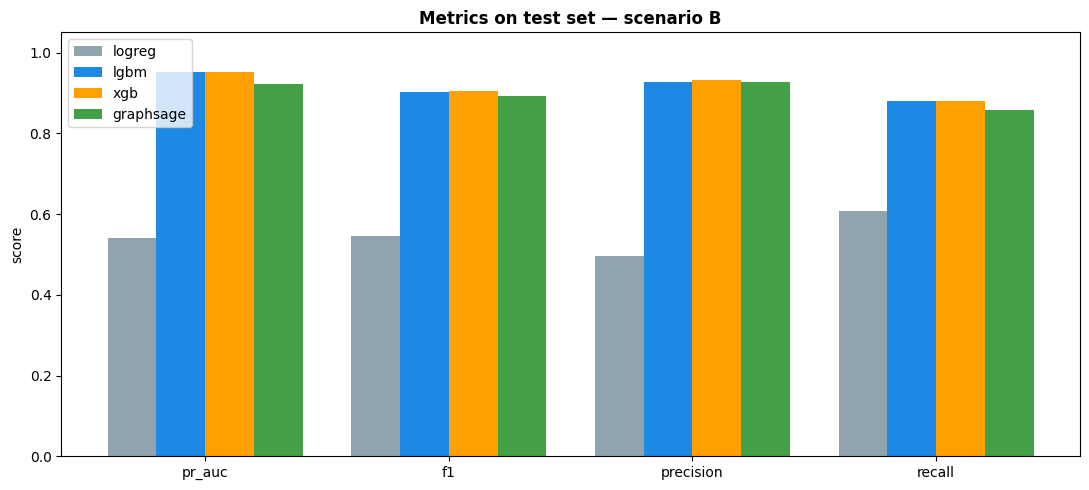
\includegraphics[width=0.78\textwidth]{stop_level/metrics_summary_B.png}
    \caption{Per-model PR-AUC, F1, precision and recall on the test set under scenario~B. Tree- and graph-based models cluster above \num{0.92}; logreg saturates lower.}
    \label{fig:metrics-summary}
\end{figure}

\paragraph{Calibration.} Post-isotonic test ECE is below \num{0.002} for all four tree models (LightGBM~A \num{0.001}, LightGBM~B \num{0.000}, XGBoost~A \num{0.002}, XGBoost~B \num{0.000}). Logistic regression scenario~A retains ECE \num{0.076}: a residual the linear model's lower information capacity cannot smooth out.

\subsection{Per-country and cascading-respect breakdowns}

\begin{table}[H]
    \centering
    \caption{XGBoost / scenario B, test PR-AUC and F1 by country. Finland advantage: short, recurrent runs whose \texttt{train\_station\_lag7\_rate} is highly predictive.}
    \label{tab:per-country}
    \footnotesize
    \begin{tabular}{l S[table-format=7.0,group-separator={,}] S[table-format=1.3] S[table-format=1.3]}
        \toprule
        Country & {n\_test} & {PR-AUC} & {F1} \\
        \midrule
        Finland     &  495040 & 0.990 & 0.961 \\
        Italy       &  421971 & 0.871 & 0.790 \\
        Netherlands & 1789432 & 0.857 & 0.805 \\
        \bottomrule
    \end{tabular}
\end{table}

\paragraph{Cascading respect (B/XGB).} Conditioning on the previous stop's actual disruption label,
$P(\hat{y}=1 \mid y_{k-1}=1)=\num{0.938}$ versus $P(\hat{y}=1 \mid y_{k-1}=0)=\num{0.005}$, gap $=\num{0.933}$. The model uses the inflight signal aggressively and correctly.

\paragraph{Operating points.} XGBoost~B is operationally usable as a high-precision triage signal: precision at recall \num{0.70} reaches \num{0.985}; at recall \num{0.95} it is still \num{0.548} (compared to \num{0.179} for XGBoost~A at the same recall). Performance is flat across route-position quartiles -- per-quartile PR-AUC stays in $[\num{0.935}, \num{0.954}]$.

\section{Explainability and lag-feature ablation}
\label{sec:xai}

\subsection{Setup}

We pick the strongest tabular model per scenario by test PR-AUC -- XGBoost wins both -- and run TreeSHAP~\cite{lundberg2017unified,lundberg2020local} on a stratified \num{270644}-row sample (\SI{10}{\percent} of the test set, seed~42). The lag-feature ablation refits and predicts on the full training and test sets. The full Phase~4 pipeline (both scenarios + ablation + 14 figures + a JSON report) runs in roughly 24 minutes.

\subsection{Top-5 SHAP features per scenario}

\begin{table}[H]
    \centering
    \caption{Top-5 features by mean $|\text{SHAP}|$, XGBoost test sample. Scenario~A leans on (train, station) rolling reliability and station-static history; scenario~B is dominated by the previous stop's actual delay (\num{2.464}, $\sim$3.7$\times$ the next-strongest feature).}
    \label{tab:shap-top5}
    \footnotesize
    \begin{tabular}{r l S[table-format=1.3] | l S[table-format=1.3]}
        \toprule
        \# & Scenario A feature & {mean $|\text{SHAP}|$} & Scenario B feature & {mean $|\text{SHAP}|$} \\
        \midrule
        1 & \texttt{train\_station\_lag7\_rate} & 1.061 & \texttt{prev\_stop\_actual\_delay}    & 2.464 \\
        2 & \texttt{avg\_historical\_delay}     & 0.396 & \texttt{stop\_order}                  & 0.674 \\
        3 & \texttt{stop\_order}                & 0.273 & \texttt{train\_station\_lag7\_rate}   & 0.375 \\
        4 & \texttt{station\_lag7\_rate}        & 0.194 & \texttt{max\_actual\_delay\_so\_far}  & 0.363 \\
        5 & \texttt{temperature}                & 0.165 & \texttt{avg\_historical\_delay}       & 0.297 \\
        \bottomrule
    \end{tabular}
\end{table}

\begin{figure}[H]
    \centering
    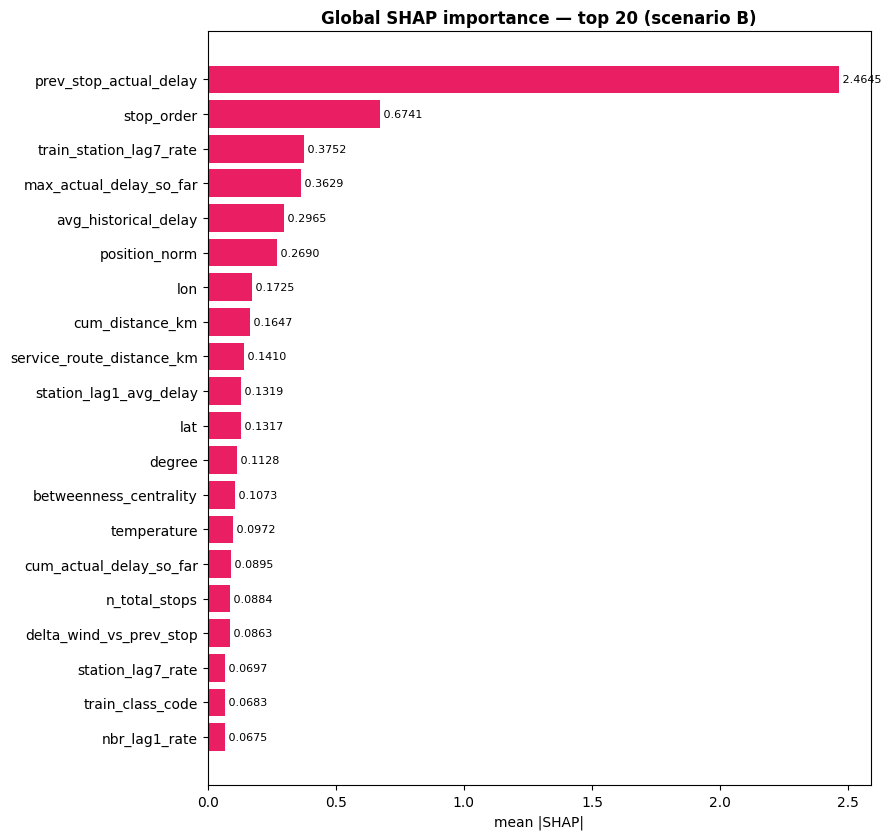
\includegraphics[width=0.78\textwidth]{xai/global_summary_bar_B.png}
    \caption{Top-20 global feature importance, scenario~B (mean $|\text{SHAP}|$). \texttt{prev\_stop\_actual\_delay} dominates by a factor of $\sim$3.7 over \texttt{stop\_order}; the historical predictors stay in the top 10 with materially lower weight.}
    \label{fig:shap-bar-B}
\end{figure}

\subsection{Lag-feature ablation}

To quantify how much of the test-set signal lives in the lag and inflight feature groups, we re-fit the winning model after removing every \texttt{*\_lag*} feature \emph{and} the three inflight features simultaneously. The remaining feature set is purely static, weather and position. The two scenarios collapse to PR-AUC \num{0.350} (\cref{tab:lag-ablation}) -- so the entire A$\to$B uplift is carried by lag and inflight features.

\begin{table}[H]
    \centering
    \caption{Lag-feature ablation. The marginal contribution of the three inflight features is +\num{0.412} test PR-AUC, almost all of it carried by \texttt{prev\_stop\_actual\_delay}.}
    \label{tab:lag-ablation}
    \footnotesize
    \begin{tabular}{l S[table-format=1.3] S[table-format=1.3] S[table-format=1.3]}
        \toprule
        Scenario & {PR-AUC (full)} & {PR-AUC (no lag/inflight)} & {$\Delta$} \\
        \midrule
        A & 0.533 & 0.350 & 0.183 \\
        B & 0.940 & 0.350 & 0.590 \\
        \bottomrule
    \end{tabular}
\end{table}

\begin{figure}[H]
    \centering
    
\includegraphics[width=0.55\textwidth]{xai/lag_ablation.png}
    \caption{Lag-feature ablation, scenario~B. Removing every lag feature and the three inflight features drops PR-AUC by \num{0.590} -- back to a static-features-only baseline.}
    \label{fig:lag-ablation}
\end{figure}

\subsection{Scenario uplift}

The per-row scenario uplift $\Delta P = P_B - P_A$ has \emph{mean} $-\num{0.128}$ on the test set (\cref{fig:uplift}). The negative sign is the right reading: scenario~A over-predicts using conservative lag/weather priors; scenario~B sees the actual prior-stop delay and revises \emph{downward} whenever that delay is small (the modal case). The effect strengthens late in the route ($-\num{0.153}$ for \texttt{position\_norm}~$\geq\num{0.75}$ vs.~$-\num{0.108}$ for \texttt{position\_norm}~$<\num{0.25}$) as B accumulates more inflight evidence.

\begin{figure}[H]
    \centering
    
\includegraphics[width=0.78\textwidth]{xai/scenario_uplift_map.png}
    \caption{Per-row scenario uplift $P_B - P_A$ vs.\ \texttt{position\_norm}. Mean uplift $-\num{0.128}$; the negative sign means B is generally \emph{more} selective than A, and the effect strengthens late in the route.}
    \label{fig:uplift}
\end{figure}

\paragraph{Take-away.} Lag features carry the +\num{0.183} A-uplift over a static baseline; the three inflight features carry an additional +\num{0.407} on top -- almost entirely via \texttt{prev\_stop\_actual\_delay}, which contributes up to $+\num{8.43}$ SHAP units on highest-confidence true positives. Within-run delay propagation is highly Markovian.

\section{Knowledge graph and cause classifier}
\label{sec:kgcause}

\subsection{Knowledge graph}

\paragraph{Why.} The four-model benchmark and the SHAP report deliver per-row probabilities and per-row attributions. Both are useful but neither answers \emph{why is this stop on the high-risk list?} That question requires graph-shaped context: the station's reliability history, recent fault reports, the immediate neighbours on the network. We therefore promote the Phase~1/2 outputs to a queryable graph database.

\paragraph{Backend.} Sparksee~5.2.3~\cite{sparksee2024,martinez2017dex}, sourced from Maven Central as \texttt{com.sparsity:sparkseejava:5.2.3}. We drive its native Java API from Python via JPype1. A one-shell-command installer (\texttt{scripts/install\_sparksee.sh}) downloads the jar plus a portable Eclipse Temurin~17 JDK into a project-local \texttt{.tools/} directory; no system-level Java install is required. Built on a Tesla~T4 + 4-core CPU host.

\paragraph{Schema.} Three node types and three edge types:
\begin{itemize}
    \item \textbf{Nodes}: \texttt{Station}(station\_id PK, country, lat, lon, avg\_historical\_delay, degree); \texttt{TrainService}(service\_id PK, country, train\_class\_code, date, is\_disrupted); \texttt{FaultEvent}(fault\_id PK, date, description).
    \item \textbf{Edges}: \texttt{STOPS\_AT} (TrainService $\to$ Station, with delay\_minutes + weather\_*); \texttt{ADJACENT\_TO} (Station $\to$ Station, distance\_km); \texttt{REPORTED\_AT} (FaultEvent $\to$ Station).
\end{itemize}

\paragraph{Bridge query.} After the SHAP report flags a high-risk stop, the analyst plugs its $(\texttt{service\_id}, \texttt{station\_id}, \texttt{date})$ triple into the bridge query, which returns: this stop's actual delay and weather, recent fault events at this station ($\leq$~14 days), and the 1-hop adjacent stations. The native \texttt{Graph.findEdge} / \texttt{Graph.neighbors} implementation in \texttt{stop\_level/build\_kg.py::run\_bridge\_demo} answers in \SI{7.7}{ms} on the FI\_HKH hub subgraph -- responsive enough to drop into an interactive disruption-monitoring dashboard.

\paragraph{Evaluation-mode cap.} The Maven Central jar runs Sparksee in \emph{personal evaluation} mode unless a licence string is provided in \texttt{sparksee.cfg}, capping each edge type at one million entries. The build script auto-falls back to a hub subgraph centred on FI\_HKH (\num{16434} TrainService, \num{98508} STOPS\_AT, \num{4} ADJACENT\_TO edges, \SI{11}{MB} on disk). Holders of a Sparksee licence can drop their string into \texttt{sparksee.cfg} and re-run with the same code path to load the full \num{16600169}-edge graph.

\subsection{Cause classifier (Netherlands)}

\paragraph{Labelled data.} The Netherlands publishes a separate disruption-incident log tagged with nine \texttt{cause\_group} classes (\emph{rolling stock, infrastructure, external, accidents, unknown, logistical, engineering work, staff, weather}). We join each disrupted Dutch stop to the most-frequent \texttt{cause\_group} reported at the same station on the same date, yielding \num{126810} labelled stops -- \SI{32.2}{\percent} of all Dutch disrupted stops. The class distribution is severely skewed: \emph{rolling stock} \SI{38.5}{\percent}; \emph{weather} \SI{1.1}{\percent}.

\paragraph{Design choices.} (i)~23 cause-specific features: peak-hour / weekend / season flags, log-transformed delay, severe-delay flags ($>$\,30/60\,min), cascade indicators from \texttt{prev\_stop\_actual\_delay}, severe-weather flags (\texttt{weather\_severity} $\geq 3$ and $=4$), a heavy-snow flag, and the interaction \texttt{winter\_x\_severe\_weather}. (ii)~Symmetric \texttt{compute\_sample\_weight('balanced')} passed to all base models. (iii)~Boosted models use 800 trees, deeper splits and L1/L2 = \num{0.1}. (iv)~A logreg meta-stacker over five base models.

\paragraph{Headline.} LightGBM is the test winner: macro-F1 $=\num{0.213}$. The stacker leads on validation but overfits to \num{0.137} on test -- a textbook example of why a separate held-out is needed when meta-learning is involved. The most striking single result is the rare \emph{weather} class at F1$=\num{0.509}$, attributable to the \texttt{winter\_x\_severe\_weather} interaction; without it the model never predicts \emph{weather} at all.

\begin{table}[H]
    \centering
    \caption{Selected per-class test F1 for the winning LightGBM cause classifier on the Dutch test set (test rows: \num{19913}; macro-F1 \num{0.213}).}
    \label{tab:cause}
    \footnotesize
    \begin{tabular}{l S[table-format=4.0,group-separator={,}] S[table-format=1.3] l}
        \toprule
        Class & {Support} & {F1} & Comment \\
        \midrule
        \textbf{weather}  &  111 & {\bfseries 0.509} & carried by \texttt{winter\_x\_severe\_weather} \\
        rolling stock     & 7376 & 0.425 & no longer the default class \\
        staff             &  743 & 0.377 & distinctive temporal pattern \\
        infrastructure    & 6536 & 0.253 & \\
        external          & 2455 & 0.165 & \\
        engineering work  &  235 & 0.000 & overlaps temporally with \emph{logistical} \\
        \bottomrule
    \end{tabular}
\end{table}

\subsection{Cross-country transfer (no fine-tuning)}

We apply the winning Dutch classifier to \num{340319} disrupted Italian stops and \num{865560} disrupted Finnish stops without retraining. \textbf{Italy} (mean confidence \num{0.600}, trust 3/10) collapses onto \emph{engineering work} (\SI{54.8}{\percent}) -- a class on which the model scores F1$=\num{0.000}$ within the Netherlands. Root cause: \texttt{lib\_italy.py:204} zero-fills missing weather columns, so the cause classifier interprets the all-zero \texttt{temperature} column as ``extreme winter conditions''. \textbf{Finland} (mean confidence \num{0.369}, trust 4/10) produces a domain-plausible distribution dominated by \emph{infrastructure} (\SI{30.2}{\percent}) and \emph{external} (\SI{30.0}{\percent}), consistent with published Finnish railway literature -- \textbf{but the \emph{weather} class is still missed}: only \SI{0.1}{\percent} of Finnish disrupted stops are tagged weather despite \SI{27}{\percent} having severity~$\geq 3$. Root cause: feature-scale mismatch -- Dutch \texttt{precipitation} is Open-Meteo daily mm/day, Finnish \texttt{precipitation} is FMI hourly mm/h, so the threshold the model learned on Dutch values does not fire on Finnish values.

\paragraph{Recommended fixes (in expected-lift order).} (1)~Per-country mean-variance alignment of temperature and precipitation; (2)~fix the Italian zero-fill bug (one-line change); (3)~deterministic rule for the easy case (\texttt{weather\_severity} $\geq 3$ and \texttt{snow\_depth} $\geq 15$\,cm $\Rightarrow$ weather); (4)~hierarchical cause modelling; (5)~collect a small per-country labelled set (5--10\,K rows) and fine-tune.

\section{Reproduction, limitations, future work}
\label{sec:repro}

\subsection{Reproduction in four shell commands}

\begin{verbatim}
# 1. Raw data (~5.7 GB)        # 2. Per-country preprocessing (papermill)
bash scripts/download_data.sh   bash preprocess/run_all_notebooks.sh

# 3. Unified store + benchmark + evaluation + SHAP (one chained command)
python stop_level/preprocess_stops.py
python stop_level/train_all.py \
    --model logreg lgbm xgb graphsage --scenario both \
  && python stop_level/evaluate.py \
  && python stop_level/xai_stops.py --scenario both --sample-frac 0.10

# 4. (Optional) Sparksee KG (5.2.3 jar from Maven Central + Temurin 17)
bash scripts/install_sparksee.sh && python stop_level/build_kg.py
\end{verbatim}

\paragraph{Tests.} \texttt{python -m pytest stop\_level/tests/ -q} $\to$ 30 total, 29 passing, 1 environment-skip (the \texttt{graphsage\_smoke} test when \texttt{torch\_geometric} is not installed). Suite executes in $\sim$20\,s.

\paragraph{Wall-clock.} On a multi-core CPU host (GraphSAGE + KG on a Tesla~T4), end-to-end is $\sim$1.5\,h: Phase~1 (per-country preprocessing) 18\,min; Phase~2 (feature store) 17\,min; Phase~3 (model training) 30\,min; Phase~4 (SHAP + ablation, \SI{10}{\percent} sample) 24\,min; Sparksee KG 10\,min; cause classifier 20\,min.

\paragraph{Artefact map.} After a full run the canonical consumables are: \texttt{\seqsplit{Data/stops/stops\_\{train,val,test\}.parquet}} (47 columns, scaled), \texttt{\seqsplit{feature\_names\_\{A,B\}.json}} (the contract), \texttt{\seqsplit{scaler\_\{mean,scale\}\_\{A,B\}.npy}} (inverse transform), \texttt{edge\_index.npy} + \texttt{edge\_attr.npy} (PyG-compatible station graph), \texttt{\seqsplit{stop\_level/results/benchmark\_stops.json}} (every metric table), \texttt{\seqsplit{stop\_level/results/xai\_report\_stops.json}} (SHAP global + 4 local explanations + lag-ablation + KG-bridge Cypher), and 22 figures under \texttt{stop\_level/figures/}.

\subsection{Limitations}

\begin{enumerate}
    \item \textbf{Italian zero-fill weather bug.} \texttt{lib\_italy.py:204} zero-fills missing weather columns instead of preserving \texttt{NaN}. Downstream consequence: \emph{engineering work} mode collapse on the Italian cause-classifier transfer (\cref{sec:kgcause}). One-line fix.
    \item \textbf{Sparksee evaluation-mode cap.} The Maven Central jar caps each edge type at one million entries unless a licence string is supplied; the build script auto-falls back to the FI\_HKH hub subgraph. Holders of a Sparksee licence load the full \num{16600169}-edge graph through the same code path.
    \item \textbf{Cause label coverage.} Only \SI{32.2}{\percent} of Dutch disrupted stops have a matching incident-log entry, so the labelled set is a biased subsample of the disrupted population.
    \item \textbf{Cross-country feature scales.} Open-Meteo daily aggregates and FMI hourly observations produce numerically different precipitation distributions, breaking the transfer of weather-related cause predictions to Finland.
    \item \textbf{NL Open-Meteo coverage} is 205 of 551 stations -- cross-border stations have no Open-Meteo coordinates. Tree models handle the resulting \texttt{NaN} natively; logreg imputes via per-column train medians.
    \item \textbf{Bidirectional LSTM deferred.} The architecture is sound at synthetic scale but the current packer materialises a $[\text{services}, \text{max\_stops}, F]$ tensor up front, which exceeds \SI{15}{GB} on the full Dutch data. A streaming, generator-based packer would solve this.
\end{enumerate}

\subsection{Future work}

(i)~Streaming packer to bring the BiLSTM into the benchmark; (ii)~per-country mean-variance alignment of weather feature scales to fix the Finnish weather under-prediction; (iii)~a small Italian-specific cause label collection (5--10\,K rows) to break the NL$\to$IT transfer ceiling; (iv)~hierarchical cause modelling (\texttt{cause\_group} first, then sub-cause); (v)~loading the full \num{16600169}-edge graph in Sparksee under licence, demonstrating the same code path scales without modification; (vi)~refresh \texttt{avg\_historical\_delay} from a strictly-past rolling window in production.

\subsection{Closing summary}

The unified pipeline harmonises three open European railway feeds at \num{16600169}-stop scale with a single anti-leakage Common Data Model. Four model families benchmarked twice show that XGBoost wins both scenarios: PR-AUC \num{0.527} pre-departure, \num{0.939} inflight. The lag-feature ablation shows the entire uplift is carried by lag and inflight features; SHAP shows that within scenario~B almost the whole signal is one feature, \texttt{prev\_stop\_actual\_delay}. The Sparksee~5.2.3 knowledge graph closes the loop from per-row attribution to spatial-temporal context in \SI{7.7}{ms}. The Dutch cause classifier reaches macro-F1 \num{0.213} with the rare \emph{weather} class at F1$=\num{0.509}$; cross-country transfer is documented to fail along two specific axes for which the recommended fixes are concrete and small. Reproducible from raw open data with four shell commands; 29/30 tests pass.


\bibliography{references}

\end{document}
